\section{Methods}\label{section:methods}

%% 本節では、振動抽出システムの評価方法について述べる。
In This section,describes the evaluation method of the Real-time vibration extraction system.

%% 本研究では3つの実験を行い、振動抽出システムを評価を行う。
%% なお、振動抽出システムは水平方向と垂直方向の振動成分を抽出することができるが、
%% 本研究では、垂直方向の振動成分のみを評価対象とする。
%% また、振動抽出FPGAシステムの出力は位相遅れなく振動成分を推定できる反面、
%% 振動の変位量については十分な制度が担保されていない。
%% そのため、本研究では、位相情報に着目した評価を行う。
In this study, three experiments will be conducted to evaluate the Real-time vibration extraction system.
Note that although the vibration extraction system can extract horizontal and vertical vibration components,
only the vertical vibration components will be evaluated in this study.
While the output of the vibration extraction system can estimate vibration components without phase delay,
the system does not guarantee sufficient system for the amount of vibration displacement. Therefore, in this study, the evaluation will focus on the phase information.

\subsection{Vibration extraction experiment using simulated video}\label{subsection:experiment1}
%% この実験では、CGを用いて作成された内視鏡手術の模擬映像を振動抽出システムに入力する。
%% 模擬映像はHD解像度($1280 \times 780$)、$60$FPSの約$12.5$秒間の映像であり、手術器具先端が
%% $1$Hzと$10$Hzの合成波に沿って振動する様子を再現している。
%% 模擬映像における振動データと振動抽出システムの出力結果とを比較することで、振動の抽出精度の評価を行うことができる。

In this experiment, a simulated video of endoscopic surgery created using computer graphics is input to the vibration extraction system.
The simulated video is an approximately $12.5$ second video
with HD resolution($1280 \time 780$) and $60$FPS,
reproducing the vibration of the tip of a surgical
instrument along a composite wave of $1$Hz and $10$Hz.
By comparing the vibration data in the simulated video
with the output results of the vibration extraction system,
the accuracy of vibration extraction can be evaluated.

%% この実験は、山下らが構築した検証プラットフォームを使用する\cite{bib:kensyo_eng}。
%% 山下らの検証プラットフォームはSoC FPGAによるPS-PL通信を用いることで
%% PL部に実装された実機動作するFPGA画像処理システムに対してリアルタイムな検証用動画像の入力と
%% それに対する出力値の取得を可能にし,この出力値から実機動作するFPGA画像処理システムの
%% 定量的評価を行える検証環境である.
%% この検証プラットフォームを使用することにより,検証対象システムに大きな変更を加えることなく
%% 最小限の手順で画像処理システムの定量的評価を行うことが可能である.

This experiment uses the verification platform built by Yamashita et al.\cite{bib:kensyo_eng}
Yamashita et al.'s verification platform uses SoC FPGA PS-PL communication
to enable real-time input of verification videos to the FPGA image processing system
implemented in the PL section and acquisition of output values in response to these inputs.
This verification environment enables quantitative evaluation
of FPGA image processing systems running on actual machines.
Using this verification platform, quantitative evaluation of
image processing systems can be performed in a minimum number of steps
without making major changes to the system under verification.

%% また、振動抽出システムにはいくつかのパラメータがあり、パラメータの値によって振動の抽出精度が左右される。そこで、システムのパラメータを変更しながら複数回実験を行い、パラメータ値が、抽出精度にどれほどの影響を与えるか評価する。

The vibration extraction system has several parameters,
and the accuracy of vibration extraction depends on the parameter values.
Therefore, we will conduct several experimentswhile changing the parameters
of the system and evaluate how much the parameter values affect the extraction accuracy.



\subsection{Vibration experiments using a vibratory apparatus}\label{subsection:add_experiment}

\begin{figure}[tb]
  \centering
  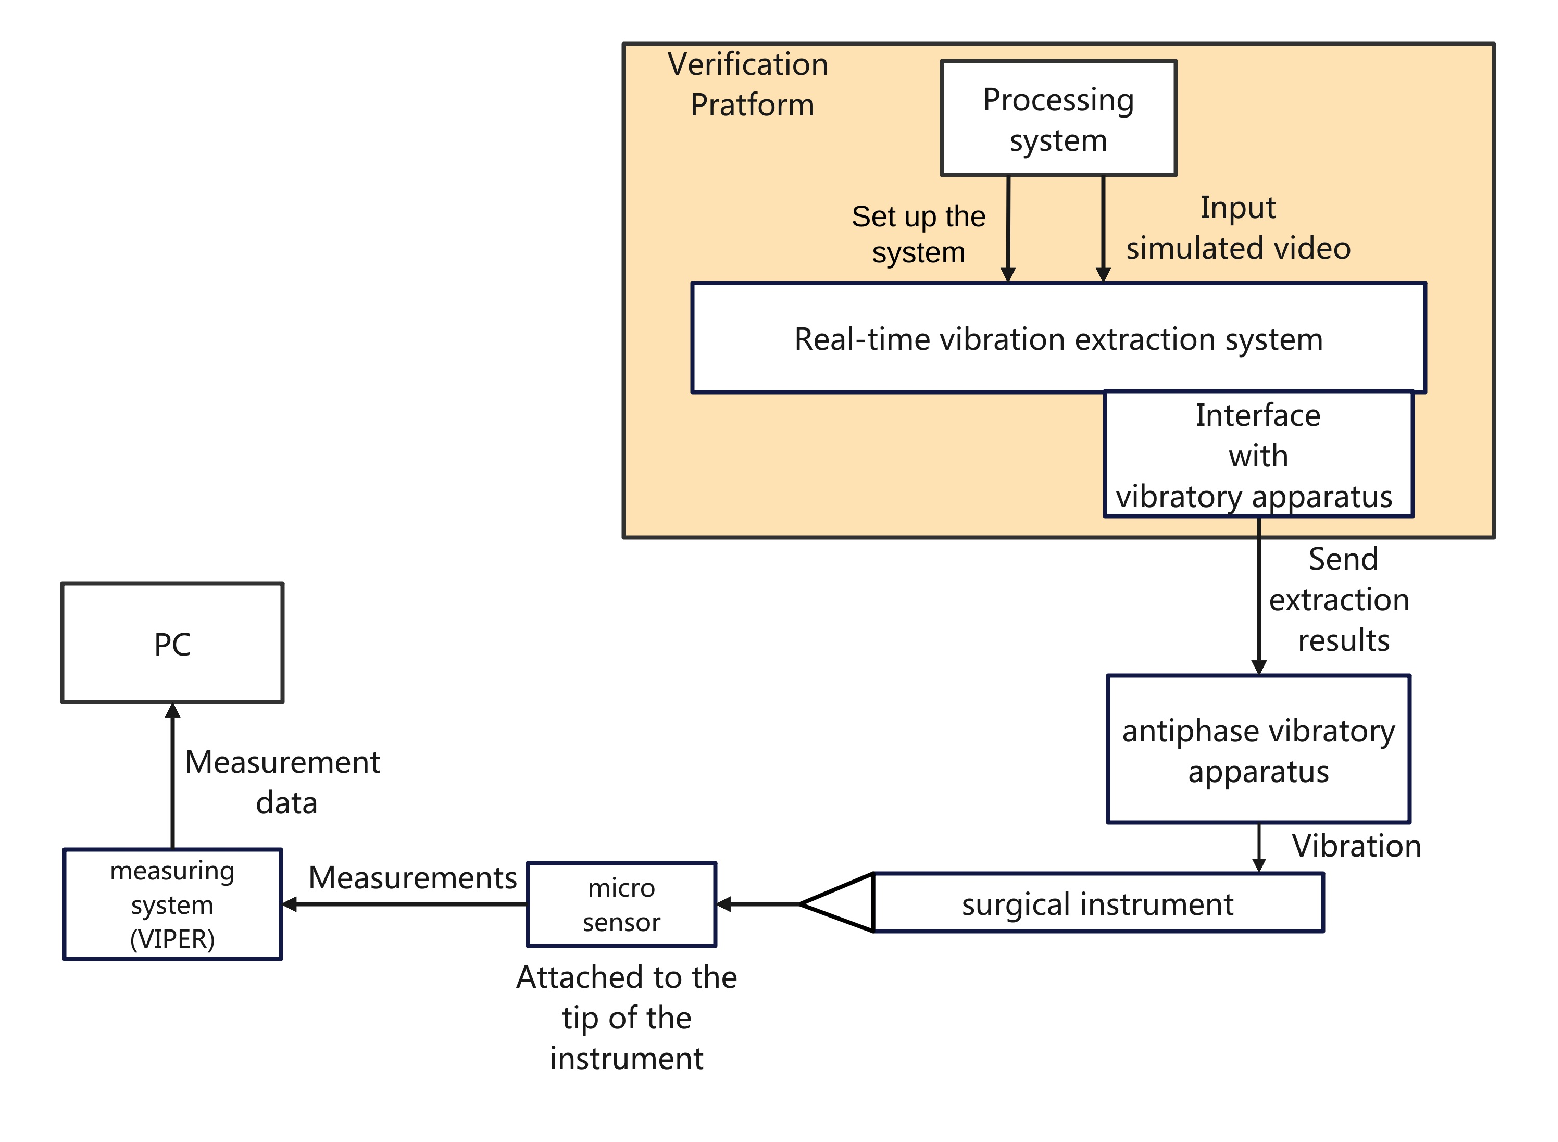
\includegraphics[width = 8cm,pagebox=cropbox,clip]{img/vibration_test.pdf}
  \caption{vibration experiments}
  \label{figure:vibration_test}
\end{figure}


\begin{table}[tb]
  \centering
  \caption{Communication standard with antiphase vibratory apparatus}
  \label{table:interface}
  \begin{tabular}{|c|l|c|}
    %%\toprule
    \hline
    Number & Data & Summary                                         \\ \hline \hline
    %% \midrule
    1 &          0xFF            &   Header                         \\ \hline \hline
    2 & Frame Number( 1〜 8bits) &  Current frame number            \\ \cline{1-2}
    3 & Frame Number( 9〜16bits) &  (Transmitted 8 bits at a time   \\ \cline{1-2}
    4 & Frame Number(17〜24bits) &   starting with the lower bits)  \\ \cline{1-2}
    5 & Frame Number(25〜32bits) &                                  \\ \hline \hline
    6 & Movement Postion( 1〜 8bits)  &  Relative position from the    \\ \cline{1-2}
    7 & Movement Postion( 9〜16bits)  &  start of inhibition ($\mu$m)  \\ \cline{1-2}
    8 & Movement Postion(17〜24bits)  &  (Transmitted 8 bits at a time \\ \cline{1-2}
    9 & Movement Postion(25〜32bits)  &  starting with the lower bits) \\ \hline
    %% \bottomrule
  \end{tabular}
\end{table}



%% この実験では、振動抽出システムと逆位相波加振装置を接続し、
%% 手術器具への加振のテストを行う。
%% この実験の概要を図\ref{figure:vibration_test}に示す。
%% 検証プラットフォームを用いて振動抽出システムに模擬映像を入力する。
%% 抽出結果を加振装置に入力し、手術器具の模型に加振する。
%% 加振精度の評価を行うため、本実験でのみ逆位相の振動ではなく正位相の振動を加振する。
%% その様子を3次元位置測定システムのVIPER\cite{bib:VIPER}を用いて計測する。
%% この計測データを用いて評価を行う。
%% 逆位相波加振装置との通信は表\ref{table:interface}に示す規格に従った。
%% 一回の通信で、ヘッダー、フレームナンバー、手術器具の先端を移動させる位置のデータを送信する。
%% 移動位置は、振動抽出開始時の位置からの相対位置を送信する。
%% この実験を行うにあたり、逆位相波加振装置とのインタフェースをRTLで実装した。
%% 振動抽出システムは1フレームの処理が完了すると、垂直方向の振動成分の抽出結果と、送信開始の信号をインタフェースに入力する。
%% インタフェースは送信開始の信号を受け取ると、表\ref{table:interface}
%% の規格通りにデータを送信する。
%% 今回は位相情報に着目した評価を行うため、振動抽出システムの抽出結果の符号のみを参考に、抽出振動の変位量を固定値(Const\_Value)に変換する。
%% 固定値に変換した抽出データから、抽出データの累積値を計算する。この累積値が振動抽出開始時の位置からの相対位置となる。
%% 次に移動平均フィルタを用いて低周波成分を除去する。
%% これは、予備実験にて累積値が時間の経過とともにマイナス方向にトレンドすることが判明したためである。
%% このトレンド成分を除去するために、ローパスフィルタとして移動平均フィルタ
%% を採用している。
%% 逆位相波加振装置へは、シリアル通信(RS232-C)でデータを送信する。


In this experiment, a vibration extraction system is connected
to a antiphase vibratory apparatus to test the excitation to the surgical instruments.
An overview of this experiment is shown in Figure \ref{figure:vibration_test}.
Input the simulated video to the vibration extraction system using the validation platform.
The extraction results are input to the vibratory apparatus and vibrations are applied to the model of the surgical instrument.
In order to assess the accuracy of the vibration excitation, positive-phase vibration is applied instead of reverse-phase vibration only in this experiment.
The situation is measured using the electromagnetic motion tracking system, VIPER\cite{bib:VIPER}.
This measurement data is used for evaluation.
The communication with the antiphase vibration apparatus followed the
standard shown in table \ref{table:interface}.
In a single communication, the header, frame number,
and data on the position at which the tip of the surgical instrument is
to be moved are transmitted.
The position to be moved is transmitted relative to the position
at the start of vibration extraction.

To conduct this experiment, an RTL implementation of an interface
to an inverse phase wave excitation system was used.
When the vibration extraction system completes processing one frame,
it inputs the result of the extraction of the vertical vibration
component and the signal to start transmission to the interface.
When the interface receives the signal to start transmission,
it transmits the data as per the standard in the table \ref{table:interface}.
In order to evaluate this time focusing on phase information, the amount of displacement of the extracted vibration is converted to a fixed value (Const\_Value)、with reference only to the sign of
the extraction result of the vibration extraction system.
From the extracted data converted to fixed values,
the cumulative value of the extracted data is calculated.
This accumulated value is the position relative to the position at the start of vibration extraction.
Next, a moving average filter is used to remove low-frequency components.
This is because preliminary experiments have shown that the cumulative values trend
in a negative direction over time, as shown in figure\ref{figure:drift_plot}.
This is because preliminary experiments have shown that the accumulated values trend
in a negative direction over time.
To remove this trend component, a moving average filter is employed as a low-pass filter.
Data is sent to the antiphase vibratory apparatus via serial communication (RS232-C).


\begin{figure}[tb]
  \centering
  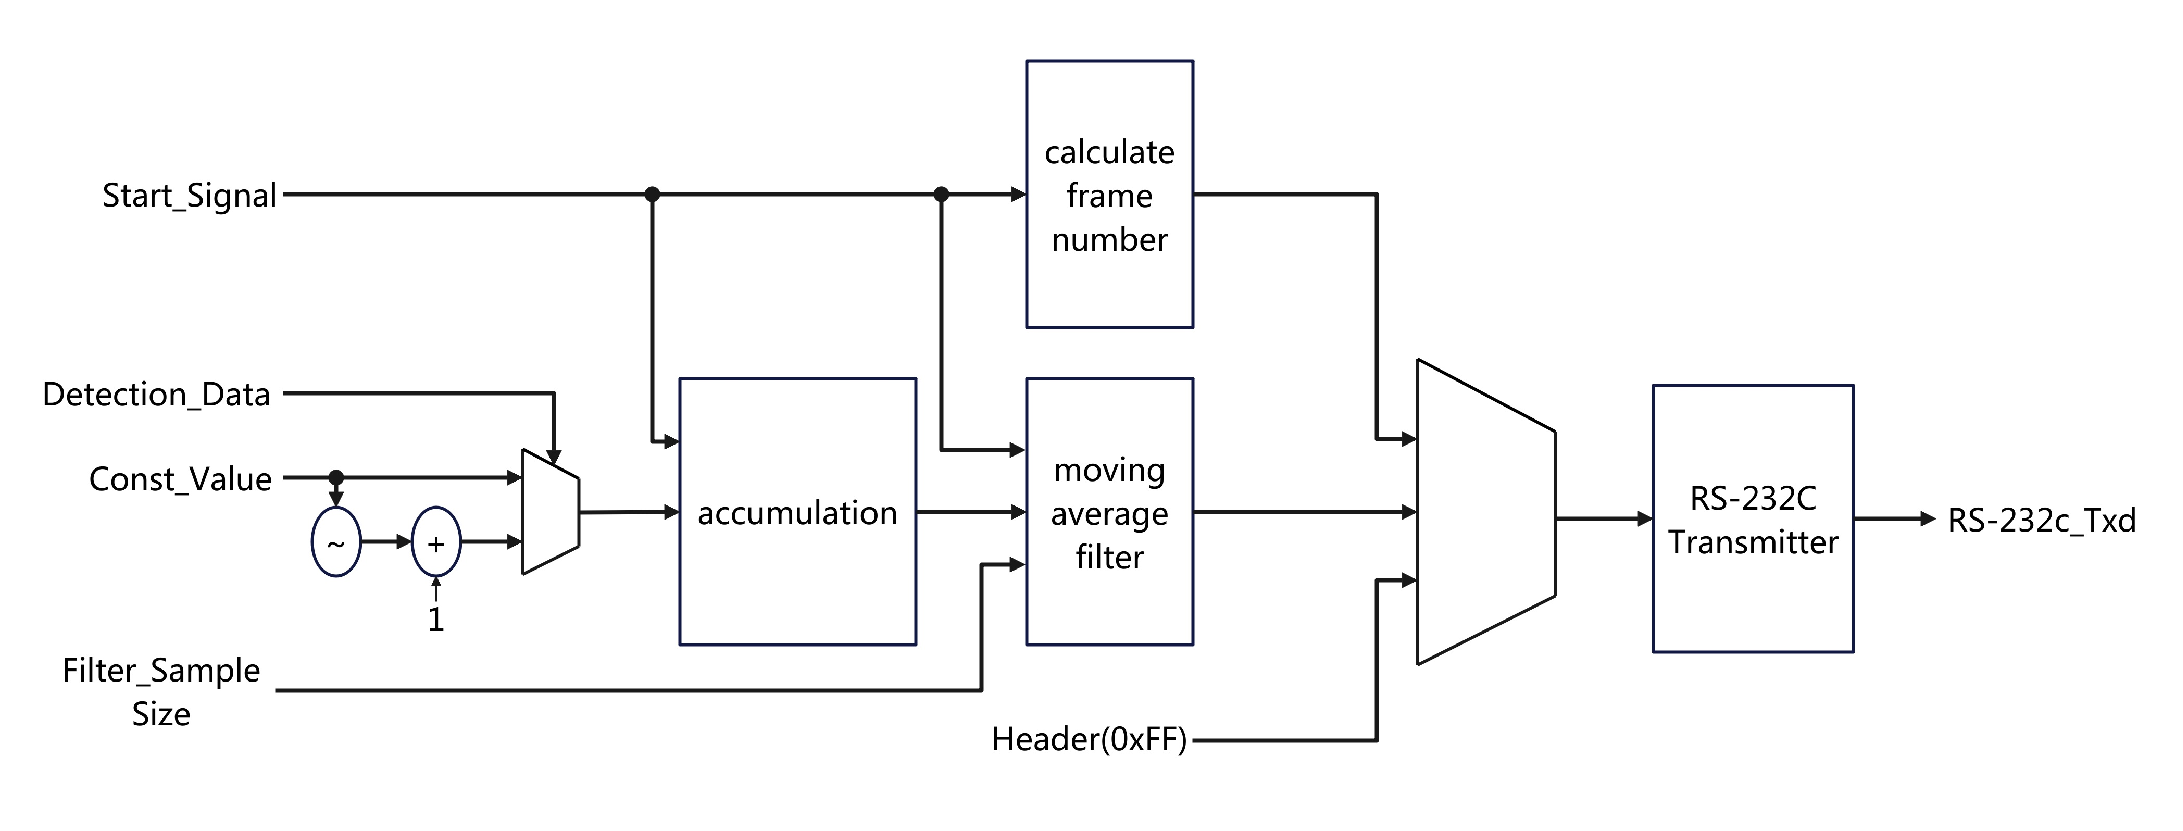
\includegraphics[width = 10cm,pagebox=cropbox,clip]{img/interface.pdf}
  \caption{Interface with vibratory apparatus}
  \label{figure:interface}
\end{figure}

\begin{figure}[tb]
  \centering
  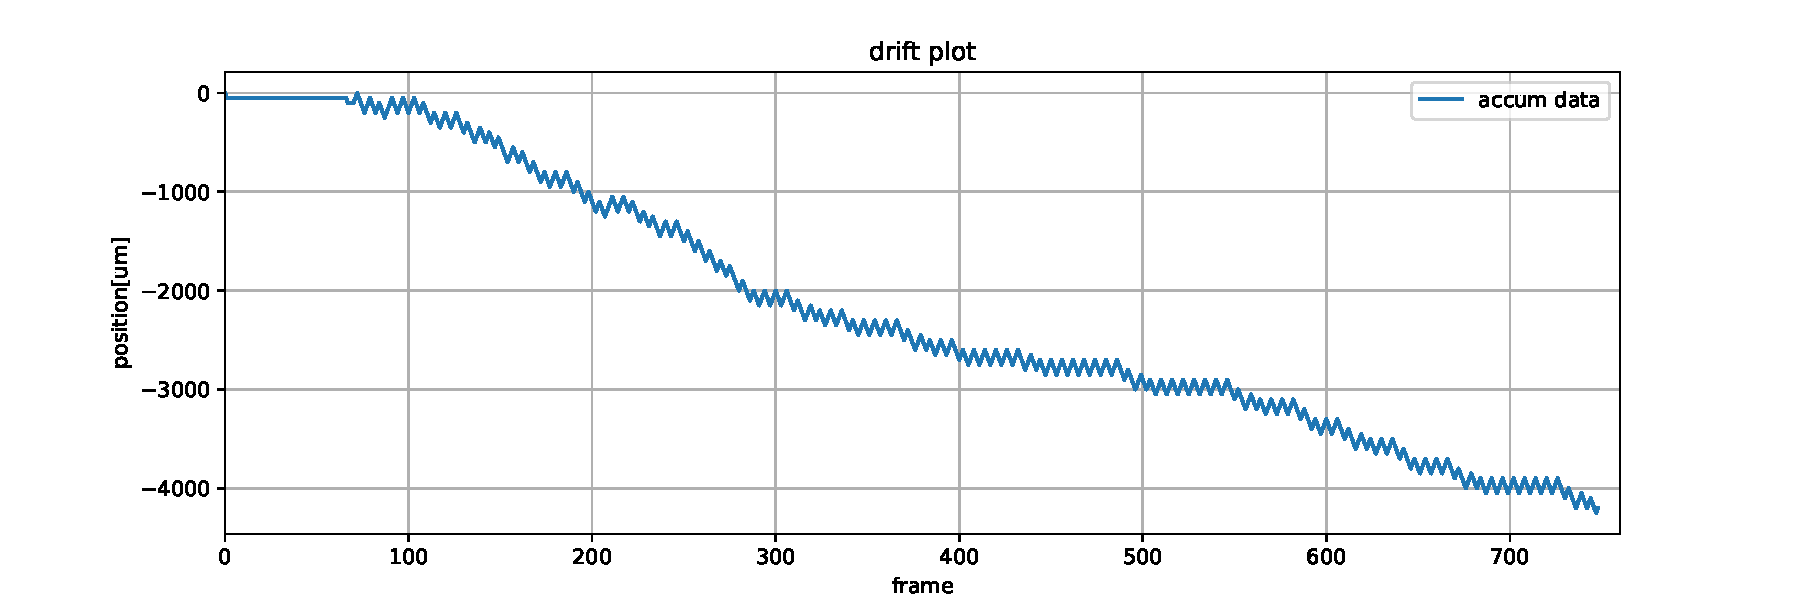
\includegraphics[width = 10cm,pagebox=cropbox,clip]{img/drift_plot.pdf}
  \caption{Cumulative value of extraction results}
  \label{figure:drift_plot}
\end{figure}




\subsection{ Tremor suppression experiment using a tremor reproduction device}\label{subsection:suppression_experiment}

%% この実験では田中らが開発した振戦再現装置\cite{bib:tremor_reproduction}を用いて振戦振動を手術器具に再現し、
%% その振動を振戦抽出システムと逆位相波加振装置を用いて抑制する。
%% 振戦再現装置は手術器具の模型をヒトが手に持った際の手術器具先端の振戦を含む振動を測定し,測定した振動を高精度に再現する.

%% この実験の概要を図\ref{figure:suppression_test}に示す。
%% まず、振戦再現装置を用いて手術器具の模型に0 Hzの定常波の振戦振動を再現する。
%% その振動を顕微鏡カメラで捉え、撮影した映像をリアルタイムで振動抽出システムに入力して振戦振動を
%% 抽出する。
%% 抽出した振動情報をもとに逆位相波加振装置で振動抑制を行い、その様子VIPERで計測し評価を行う。
%% 今回の実験では、10 Hzの定常波を手術器具の模型


In this experiment, the vibration reproduction device developed by Tanaka et al.\cite{bib:tremor_reproduction_eng}
is used to reproduce the vibration of the surgical instrument,
and the vibration is suppressed using a vibration extraction system and
an antiphase wave apparatus. The vibration reproducer measures vibrations,
including tremors at the tips of surgical instruments when a human holds a model of a surgical instrument in his/her hand,
and reproduces the measured vibrations with high precision. An overview of this experiment is shown in Figure \ref{figure:suppression_test}.
First, vibrations are reproduced on a model of a surgical instrument using a vibration reproduction device.
First, a vibration reproduction device is used to reproduce a 10 Hz stationary wave of tremor vibration
on a model of a surgical instrument.
The vibrations are captured by a microscope camera, and the captured images are input to the vibration extraction system
real time to extract the vibrations. Based on the extracted vibration information,
vibration suppression is performed using an inverse phase wave shaker,
and the vibration is measured and evaluated using VIPER.



\begin{figure}[tb]
  \centering
  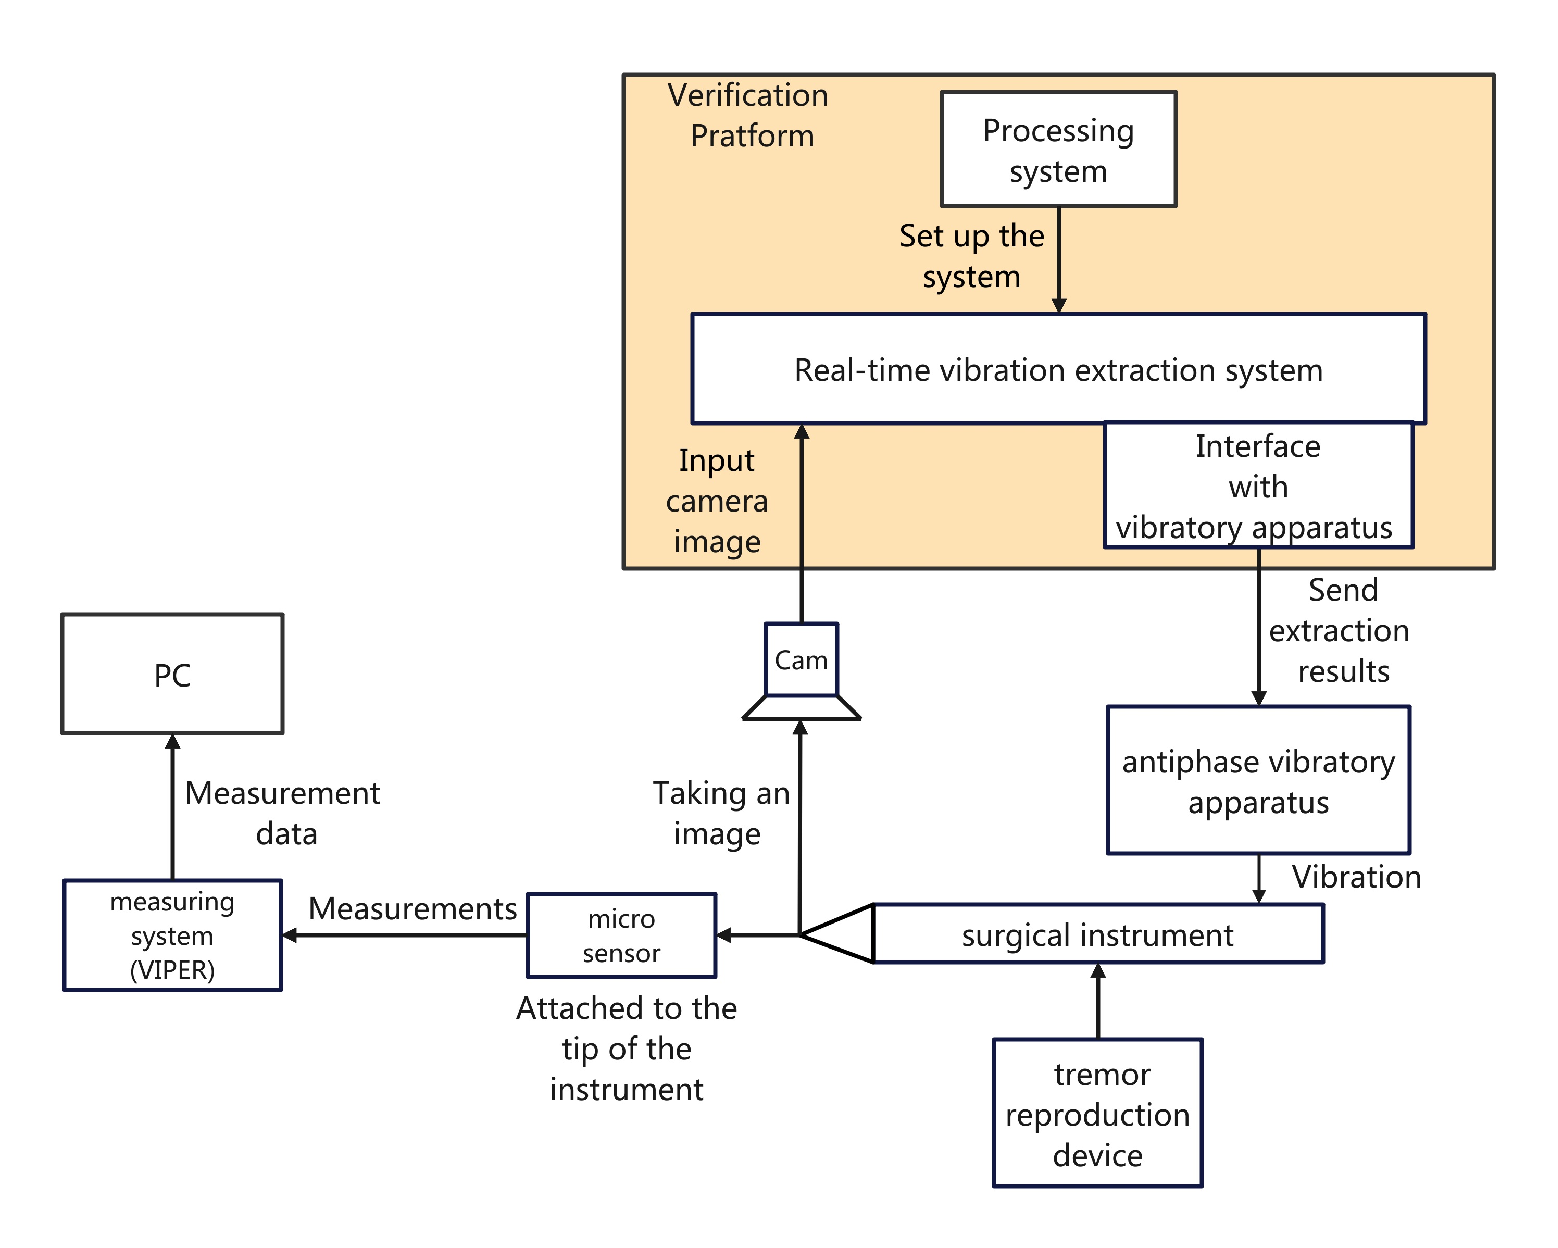
\includegraphics[width = 8cm,pagebox=cropbox,clip]{img/suppression_test.pdf}
  \caption{Cumulative value of extraction results}
  \label{figure:suppression_test}
\end{figure}
